\section{An ARX model for the heating of a box}
\label{sec:q3}

This section develops an ARX (AutoRegressive with eXogenous inputs) model for the heating power $P_h$ of an insulated box, using temperature difference $T_\Delta$ and solar irradiance $G_v$ as exogenous inputs. The data comprise 231 hourly observations from a controlled experiment.

%% 3.1 ---------------------------------------------------------------
\subsection{3.1 Time series}
\label{sec:q3_31}

Figure~\ref{fig:q3_ts} shows the three time series. The heater power $P_h$ ranges from 14 to 98\,W and exhibits clear diurnal patterns driven by both $T_\Delta$ (12.6--25.4\,$^\circ$C) and $G_v$ ($-2.2$--876\,W/m$^2$). The solar irradiance $G_v$ is zero at night and peaks during daytime, while $T_\Delta$ follows a smoother trajectory governed by ambient temperature variations.

\begin{figure}[H]
  \centering
  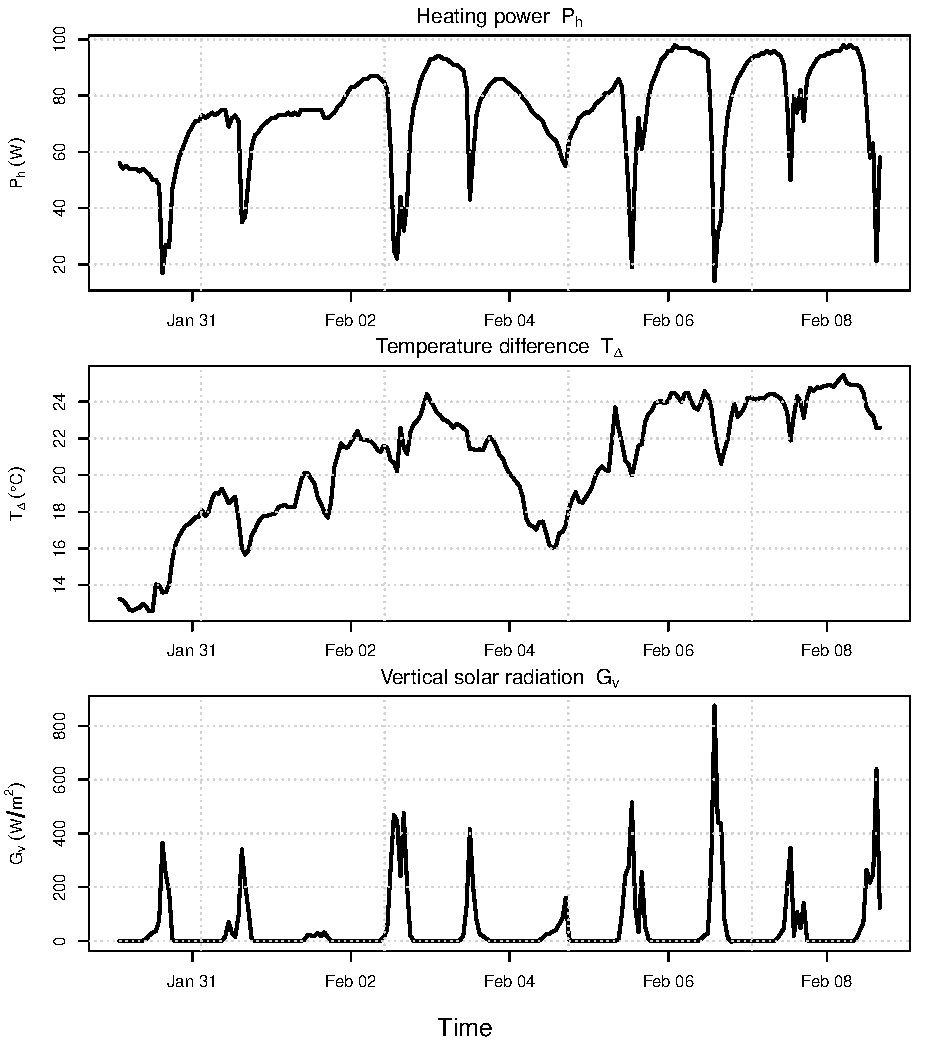
\includegraphics[width=\linewidth]{figures/q3_31_time_series}
  \caption{Hourly time series of heater power $P_h$, temperature difference $T_\Delta$, and solar irradiance $G_v$ over the 231-observation period.}
  \label{fig:q3_ts}
\end{figure}

%% 3.2 ---------------------------------------------------------------
\subsection{3.2 Train/test split}
\label{sec:q3_32}

The data are split chronologically: the first 149 observations (up to 2013-02-05 06:00) form the training set, and the remaining 82 observations form the test set. This preserves the temporal ordering required for valid time-series evaluation.

%% 3.3 ---------------------------------------------------------------
\subsection{3.3 Exploratory analysis}
\label{sec:q3_33}

Figure~\ref{fig:q3_scatter} shows scatter plots of $P_h$ against each input. The heater power increases roughly linearly with $T_\Delta$ and decreases with $G_v$, consistent with the physical interpretation: larger temperature differences demand more heating, while solar gain offsets it.

\begin{figure}[H]
  \centering
  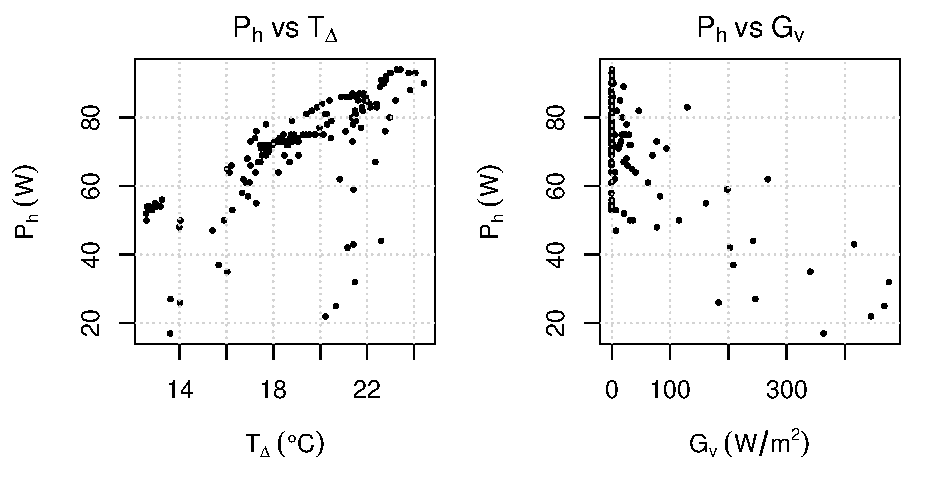
\includegraphics[width=\linewidth]{figures/q3_33_scatter}
  \caption{Scatter plots of $P_h$ versus $T_\Delta$ (left) and $P_h$ versus $G_v$ (right).}
  \label{fig:q3_scatter}
\end{figure}

The ACF of $P_h$ (Figure~\ref{fig:q3_acf_ccf}) decays slowly, indicating strong autoregressive dynamics, while the PACF cuts off sharply after lag~1--2, suggesting a low-order AR component. The raw cross-correlation functions show $T_\Delta$ positively correlated and $G_v$ negatively correlated with $P_h$ at lag~0. However, raw CCFs are biased when the input series are autocorrelated \cite[§8.7]{madsen2007time}, motivating the prewhitening analysis in Section~\ref{sec:q3_34}.

\begin{figure}[H]
  \centering
  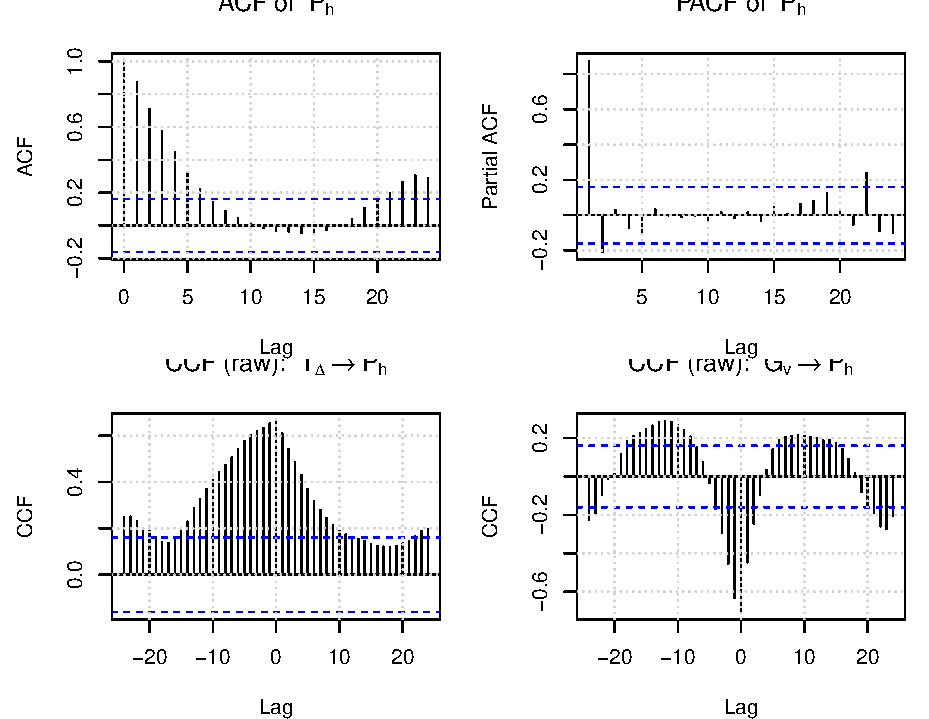
\includegraphics[width=\linewidth]{figures/q3_33_acf_ccf}
  \caption{ACF and PACF of $P_h$ (top row); raw CCF of $T_\Delta \to P_h$ and $G_v \to P_h$ (bottom row).}
  \label{fig:q3_acf_ccf}
\end{figure}

%% 3.4 ---------------------------------------------------------------
\subsection{3.4 Impulse response via prewhitening}
\label{sec:q3_34}

To obtain unbiased estimates of the impulse response, both inputs are prewhitened by fitting AR(2) models and applying the same filter to $P_h$ \cite[§8.7, p.\,269]{madsen2007time}. Figure~\ref{fig:q3_ir} shows the resulting CCFs. The $T_\Delta \to P_h$ impulse response peaks at lag~0 with $\hat{\rho} = 0.517$, and the $G_v \to P_h$ response peaks at lag~0 with $\hat{\rho} = -0.823$. Both effects are concentrated at lag~0, suggesting that the transfer function does not require delay (i.e., $b = 0$).

\begin{figure}[H]
  \centering
  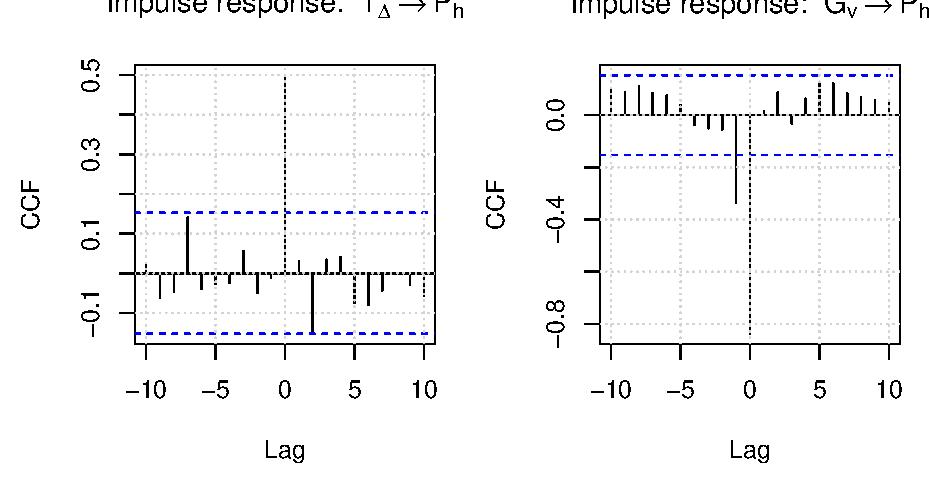
\includegraphics[width=\linewidth]{figures/q3_34_impulse_response}
  \caption{Prewhitened CCF (impulse response) for $T_\Delta \to P_h$ (left) and $G_v \to P_h$ (right).}
  \label{fig:q3_ir}
\end{figure}

%% 3.5 ---------------------------------------------------------------
\subsection{3.5 Linear regression (no AR terms)}
\label{sec:q3_35}

As a baseline, we fit a static linear regression on the training set:
\begin{equation}
  P_{h,t} = \omega_0 + \omega_1 T_{\Delta,t} + \omega_2 G_{v,t} + \varepsilon_t.
  \label{eq:lm}
\end{equation}
Both inputs are highly significant (Table~\ref{tab:lm_coef}), with $\hat{\omega}_1 = 3.42$\,W/$^\circ$C and $\hat{\omega}_2 = -0.113$\,W/(W/m$^2$), yielding $R^2 = 0.903$ and $\hat{\sigma} = 4.91$\,W. However, the residual ACF in Figure~\ref{fig:q3_lm_diag} shows strong autocorrelation, violating the i.i.d.\ assumption and indicating that AR dynamics must be included.

\begin{figure}[H]
  \centering
  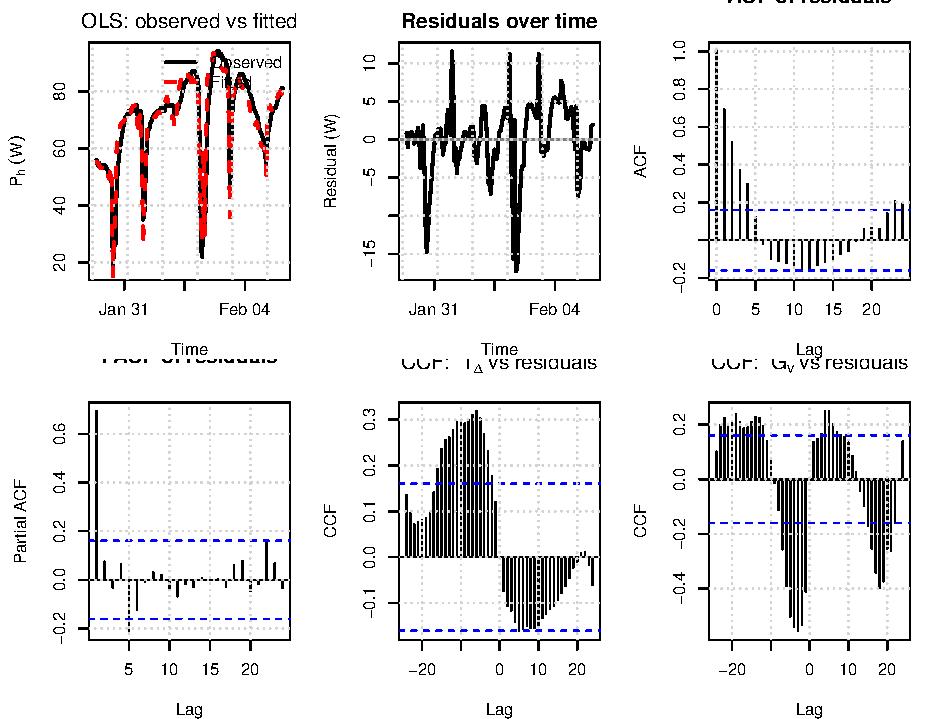
\includegraphics[width=\linewidth]{figures/q3_35_lm_diagnostics}
  \caption{Diagnostics for the static regression~\eqref{eq:lm}: fitted values, residual time series, ACF, PACF, and CCF of residuals with each input.}
  \label{fig:q3_lm_diag}
\end{figure}

\begin{table}[H]
  \centering
  % latex table generated in R 4.5.2 by xtable 1.8-8 package
% Sun Apr 12 10:43:40 2026
\begin{table}[ht]
\centering
\caption{OLS coefficient estimates for the linear regression model (3.5).} 
\label{tab:lm_coef}
\begin{tabular}{rrrrr}
  \toprule
 & Estimate & Std.\ Error & $t$-value & $p$-value \\ 
  \midrule
(Intercept) & 9.7732 & 2.6725 & 3.657 & 0.0004 \\ 
  Tdelta & 3.4212 & 0.1386 & 24.689 & 0.0000 \\ 
  Gv & -0.1131 & 0.0043 & -26.423 & 0.0000 \\ 
   \bottomrule
\end{tabular}
\end{table}

\end{table}

%% 3.6 ---------------------------------------------------------------
\subsection{3.6 ARX(1) model}
\label{sec:q3_36}

Adding one autoregressive lag gives the ARX(1) model:
\begin{equation}
  P_{h,t} = \phi_1 P_{h,t-1} + \omega_1 T_{\Delta,t} + \omega_2 G_{v,t} + \varepsilon_t.
  \label{eq:arx1}
\end{equation}
All coefficients are highly significant (Table~\ref{tab:arx1_coef}), with $\hat{\phi}_1 = 0.415$, confirming the autoregressive dynamics identified in Section~\ref{sec:q3_33}. The model achieves $R^2 = 0.977$ and $\hat{\sigma} = 2.42$\,W---a 51\% reduction in residual standard error compared to~\eqref{eq:lm}. Figure~\ref{fig:q3_arx1_diag} shows that residual autocorrelation is substantially reduced, though some structure may persist at longer lags.

\begin{figure}[H]
  \centering
  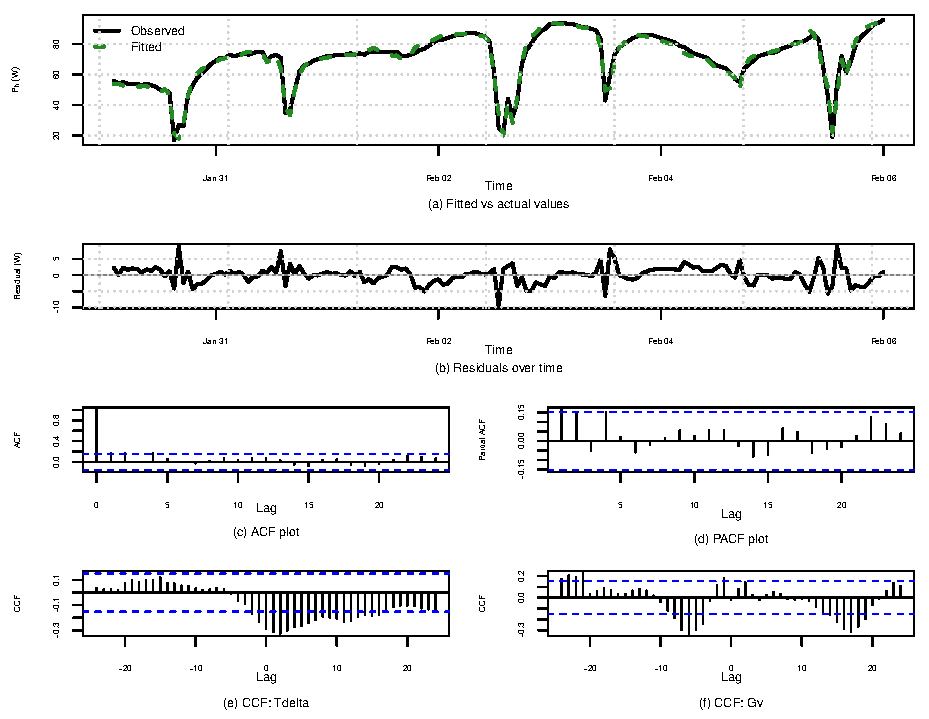
\includegraphics[width=\linewidth]{figures/q3_36_arx1_diagnostics}
  \caption{Diagnostics for the ARX(1) model~\eqref{eq:arx1}: same layout as Figure~\ref{fig:q3_lm_diag}.}
  \label{fig:q3_arx1_diag}
\end{figure}

\begin{table}[H]
  \centering
  % latex table generated in R 4.5.2 by xtable 1.8-8 package
% Sun Apr 12 10:43:40 2026
\begin{table}[ht]
\centering
\caption{OLS coefficient estimates for the ARX(1) model (3.6).} 
\label{tab:arx1_coef}
\begin{tabular}{rrrrr}
  \toprule
 & Estimate & Std.\ Error & $t$-value & $p$-value \\ 
  \midrule
(Intercept) & 4.8511 & 1.3361 & 3.631 & 0.0004 \\ 
  Ph.l1 & 0.4149 & 0.0194 & 21.378 & 0.0000 \\ 
  Tdelta & 2.0841 & 0.0926 & 22.515 & 0.0000 \\ 
  Gv & -0.0845 & 0.0025 & -33.805 & 0.0000 \\ 
   \bottomrule
\end{tabular}
\end{table}

\end{table}

%% 3.7 ---------------------------------------------------------------
\subsection{3.7 Model order selection (AIC/BIC)}
\label{sec:q3_37}

ARX models of order $p = 1, \ldots, 10$ are fitted to the training data. The general ARX($p$) model is
\begin{equation}
  P_{h,t} = \sum_{i=1}^{p} \phi_i P_{h,t-i}
           + \sum_{j=0}^{p} \omega_{1j} T_{\Delta,t-j}
           + \sum_{j=0}^{p} \omega_{2j} G_{v,t-j}
           + \varepsilon_t.
  \label{eq:arxp}
\end{equation}
Table~\ref{tab:ic} and Figure~\ref{fig:q3_aic_bic} show the information criteria. AIC selects $p = 5$ (AIC\,=\,585.8), whereas BIC selects $p = 3$ (BIC\,=\,638.6). The discrepancy arises because BIC penalises model complexity more heavily ($k \ln N$ versus $2k$), favouring a more parsimonious model.

\begin{figure}[H]
  \centering
  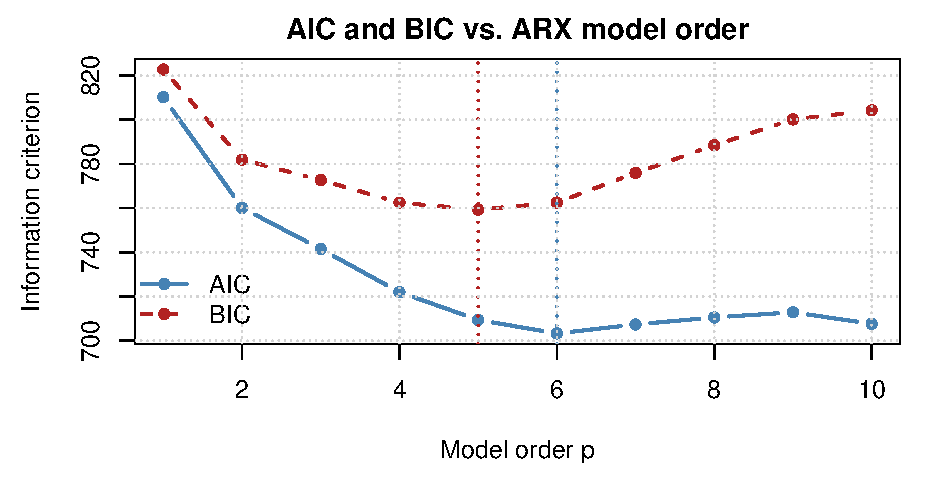
\includegraphics[width=\linewidth]{figures/q3_37_aic_bic}
  \caption{AIC and BIC as a function of ARX model order $p$.}
  \label{fig:q3_aic_bic}
\end{figure}

\begin{table}[H]
  \centering
  % latex table generated in R 4.5.2 by xtable 1.8-8 package
% Thu Apr 16 14:54:33 2026
\begin{table}[ht]
\centering
\caption{AIC and BIC for ARX models of order $p = 1, \ldots, 10$ (3.7).} 
\label{tab:ic}
\begin{tabular}{rrr}
  \toprule
Order & AIC & BIC \\ 
  \midrule
1 & 796.63 & 812.22 \\ 
  2 & 750.67 & 775.61 \\ 
  3 & 734.75 & 769.05 \\ 
  4 & 709.94 & 753.60 \\ 
  5 & 702.41 & 755.41 \\ 
  6 & 688.73 & 751.09 \\ 
  7 & 690.25 & 761.96 \\ 
  8 & 695.09 & 776.16 \\ 
  9 & 699.45 & 789.87 \\ 
  10 & 698.87 & 798.64 \\ 
   \bottomrule
\end{tabular}
\end{table}

\end{table}

%% 3.8 ---------------------------------------------------------------
\subsection{3.8 Test-set RMSE}
\label{sec:q3_38}

Figure~\ref{fig:q3_rmse} and Table~\ref{tab:rmse} report the one-step-ahead RMSE on the test set. The minimum RMSE is achieved at $p = 4$ (RMSE\,=\,3.034\,W), but the differences for $p = 2$--$5$ are negligible (range 3.03--3.06\,W). For $p \geq 6$, RMSE rises slightly, indicating overfitting. Thus the test-set criterion suggests a middle order, distinct from both AIC ($p=5$) and BIC ($p=3$).

\begin{figure}[H]
  \centering
  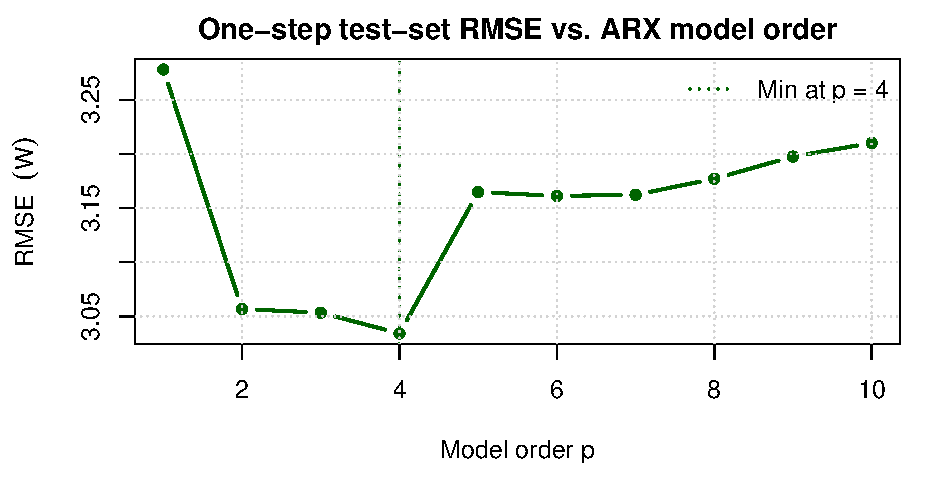
\includegraphics[width=\linewidth]{figures/q3_38_rmse}
  \caption{One-step-ahead test-set RMSE as a function of ARX model order $p$.}
  \label{fig:q3_rmse}
\end{figure}

\begin{table}[H]
  \centering
  % latex table generated in R 4.5.2 by xtable 1.8-8 package
% Sun Apr 12 10:43:41 2026
\begin{table}[ht]
\centering
\caption{One-step RMSE (W) on the test set for ARX models of order $p = 1, \ldots, 10$ (3.8).} 
\label{tab:rmse}
\begin{tabular}{rr}
  \toprule
Order & RMSE \\ 
  \midrule
1 & 3.2780 \\ 
  2 & 3.0567 \\ 
  3 & 3.0533 \\ 
  4 & 3.0341 \\ 
  5 & 3.1648 \\ 
  6 & 3.1612 \\ 
  7 & 3.1623 \\ 
  8 & 3.1771 \\ 
  9 & 3.1976 \\ 
  10 & 3.2102 \\ 
   \bottomrule
\end{tabular}
\end{table}

\end{table}

%% 3.9 ---------------------------------------------------------------
\subsection{3.9 Multi-step simulation}
\label{sec:q3_39}

We select the ARX(3) model (BIC-optimal) and evaluate its multi-step simulation performance. In simulation mode, the AR lags $P_{h,t-1}, P_{h,t-2}, P_{h,t-3}$ are computed iteratively from the model's own predictions rather than observed values, while $T_\Delta$ and $G_v$ use observed data. The full coefficient estimates are given in Table~\ref{tab:arx3_coef}.

Figure~\ref{fig:q3_sim} compares observed and simulated $P_h$ over both training and test periods. The simulation RMSE is 1.65\,W on the training set and 3.21\,W on the test set. The model tracks the diurnal heating pattern well, though accumulated prediction errors cause some drift during extended simulation. In a real-time forecasting application, the exogenous inputs $T_\Delta$ and $G_v$ would themselves need to be forecast (e.g.\ using numerical weather predictions for $G_v$), adding further uncertainty.

\begin{figure}[H]
  \centering
  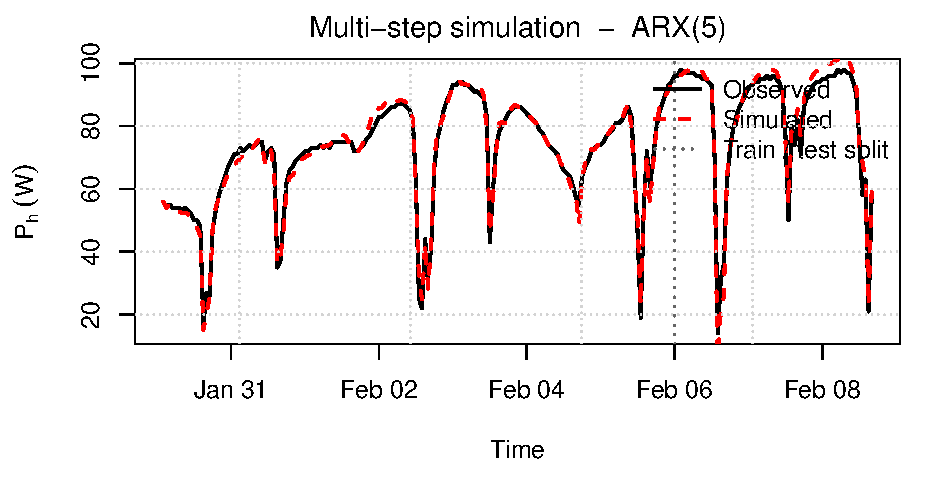
\includegraphics[width=\linewidth]{figures/q3_39_multistep_simulation}
  \caption{Multi-step simulation of the ARX(3) model: observed (black) versus simulated (red) heater power $P_h$ over the full 231-hour period.}
  \label{fig:q3_sim}
\end{figure}

\begin{table}[H]
  \centering
  % latex table generated in R 4.5.2 by xtable 1.8-8 package
% Sun Apr 19 17:00:07 2026
\begin{table}[ht]
\centering
\caption{Coefficient estimates for the chosen no-intercept ARX(3) model.} 
\label{tab:arx3_coef}
\begin{tabular}{rrrrr}
  \toprule
 & Estimate & Std.\ Error & $t$-value & $p$-value \\ 
  \midrule
Ph.l1 & 0.3784 & 0.0662 & 5.719 & 0.0000 \\ 
  Ph.l2 & 0.1823 & 0.0636 & 2.868 & 0.0047 \\ 
  Ph.l3 & -0.0007 & 0.0269 & -0.028 & 0.9781 \\ 
  Tdelta.l0 & 0.2367 & 0.3743 & 0.632 & 0.5280 \\ 
  Tdelta.l1 & 1.4960 & 0.6156 & 2.430 & 0.0162 \\ 
  Tdelta.l2 & 0.0367 & 0.4433 & 0.083 & 0.9341 \\ 
  Gv.l0 & -0.0978 & 0.0027 & -36.668 & 0.0000 \\ 
  Gv.l1 & 0.0065 & 0.0077 & 0.851 & 0.3959 \\ 
  Gv.l2 & 0.0239 & 0.0057 & 4.195 & 0.0000 \\ 
   \bottomrule
\end{tabular}
\end{table}

\end{table}

%% 3.10 --------------------------------------------------------------
\subsection{3.10 Summary}
\label{sec:q3_310}

The three selection criteria disagree: AIC selects $p = 5$, BIC selects $p = 3$, and test-set RMSE selects $p = 4$. We adopt the BIC-selected ARX(3) model as the final choice. The BIC's stronger complexity penalty guards against overfitting on this moderately sized dataset ($N = 149$), and the test-set RMSE of the ARX(3) is only marginally higher than the optimum at $p = 4$ (3.053 versus 3.034\,W). The ARX(3) model achieves a training simulation RMSE of 1.65\,W and a test simulation RMSE of 3.21\,W, demonstrating that it captures the dominant thermal dynamics of the box well.
